\documentclass[10pt]{beamer}

\usetheme[progressbar=frametitle]{metropolis}
\usepackage{appendixnumberbeamer}

\usepackage{booktabs}
\usepackage[scale=2]{ccicons}

\usepackage{pgfplots}
\usepgfplotslibrary{dateplot}

\usepackage{xspace}
\newcommand{\themename}{\textbf{\textsc{metropolis}}\xspace}

% подключаем кириллицу 
\usepackage[T2A]{fontenc}
\usepackage[utf8]{inputenc}
\usepackage{listings}
\usepackage{graphicx}
\usepackage{hyperref}
\usepackage{chronology}


\title{Metropolis}
\subtitle{A modern beamer theme}
% \date{\today}
\date{}
\author{Matthias Vogelgesang}
\institute{Center for modern beamer themes}
% \titlegraphic{\hfill\includegraphics[height=1.5cm]{logo.pdf}}






%-=-=-=-=-=-=-=-=-=-=-=-=-=-=-=-=-=-=-=-=-=-=-=-=
%        BEAMER OPTIONS
%-=-=-=-=-=-=-=-=-=-=-=-=-=-=-=-=-=-=-=-=-=-=-=-=

%\setbeameroption{show notes}

%-=-=-=-=-=-=-=-=-=-=-=-=-=-=-=-=-=-=-=-=-=-=-=-=
%
%	PRESENTATION INFORMATION
%
%-=-=-=-=-=-=-=-=-=-=-=-=-=-=-=-=-=-=-=-=-=-=-=-=

\title{Семинар 1}
\subtitle{Введение в алгоритмы. Машина Тьюринга.}
%\date{\small{\jobname}}
%\date{\today}
\author{\texttt{Бирюков Владимир}}
\institute{МФТИ}


\begin{document}

%-=-=-=-=-=-=-=-=-=-=-=-=-=-=-=-=-=-=-=-=-=-=-=-=
%
%	TITLE PAGE
%
%-=-=-=-=-=-=-=-=-=-=-=-=-=-=-=-=-=-=-=-=-=-=-=-=

\maketitle

%\begin{frame}[plain]
%	\titlepage
%\end{frame}

%-=-=-=-=-=-=-=-=-=-=-=-=-=-=-=-=-=-=-=-=-=-=-=-=
%
%	TABLE OF CONTENTS: OVERVIEW
%
%-=-=-=-=-=-=-=-=-=-=-=-=-=-=-=-=-=-=-=-=-=-=-=-=

\section{Повторение}


\begin{frame}[fragile]
\frametitle{Главные идеи первого семестра}
\begin{enumerate}
\item Язык C
\begin{enumerate}
\item Синтаксис языка C.
\item Память и указатели.
\item Сегменты памяти процесса. Стек и куча.
\end{enumerate}
\item Алгоритмы и структуры данных
\begin{enumerate}
\item Сложность алгоритмов. $O(n)$ нотация.
\item Основные структуры данных: массив, список, дерево.
\end{enumerate}
\end{enumerate}
\end{frame}


\section{Язык C}

\begin{frame}[fragile]
\frametitle{Память и указатели. Массив} 
\begin{center}
\includegraphics[width=0.95\linewidth]{images/memory_parrays_2.png}
\end{center}
\end{frame}

\begin{frame}[fragile]
\frametitle{Сегменты памяти процесса} 
\begin{center}
\includegraphics[width=0.95\linewidth]{images/process_memory_organization.png}
\end{center}
\end{frame}

\section{Алгоритмы и структуры данных}

\begin{frame}[fragile]
\frametitle{O-большое} 
\begin{center}
\includegraphics[width=0.99\linewidth]{images/On.png}
\end{center}
\end{frame}

\begin{frame}[fragile]
\frametitle{Алгоритмы сортировки}
\begin{center}
  \begin{tabular}{  l | c }
    Алгоритм сортировки & Сложность(в среднем) \\
    \hline
    Сортировка вставками & O($N^2$)\\
    Сортировка пузырьком & O($N^2$)\\
    Сортировка выбором & O($N^2$)\\
    \hline
    Сортировка слиянием & O($N\log(N)$)\\
    Быстрая сортировка & O($N\log(N)$)\\
    \hline
    Цифровая сортировка &  O($k N$) \\
  \end{tabular}
\end{center}
\end{frame}

\begin{frame}[fragile]
\frametitle{Структуры данных. Массив и связный список}
\begin{itemize}
\item Массив:\\
\quad\\
\includegraphics[width=0.8\linewidth]{images/array.png}
\item Связный список:\\
\quad\\
\includegraphics[width=0.8\linewidth]{images/list_initial.png}
\end{itemize}
\end{frame}

\begin{frame}[fragile]
\frametitle{Операции со структурами данных}
\begin{center}
  \begin{tabular}{  l | c c r }
      & Массив & Список \\
    \hline
    index & $O(1)$ & $O(N)$ \\
    find & $O(N)$ & $O(N)$  \\
    insert & $O(N)$ & $O(1)$*\\
    remove & $O(N)$ & $O(1)$*\\
    \hline
  \end{tabular}
\end{center}
* если известны указатели на данный и предыдущий элементы.
\end{frame}



\section{Машина Тьюринга}

%-=-=-=-=-=-=-=-=-=-=-=-=-=-=-=-=-=-=-=-=-=-=-=-=
%	TM: AT and definition
%-=-=-=-=-=-=-=-=-=-=-=-=-=-=-=-=-=-=-=-=-=-=-=-=


\begin{frame}{Машина Тьюринга}
\begin{columns}
\begin{column}{.48\linewidth}
Машина Тьюринга (МТ) — математическая абстракция, представляющая вычислительную машину общего вида. Была предложена 		Аланом Тьюрингом в 1936 году для формализации понятия алгоритма.
\end{column}
\begin{column}{.48\linewidth}
		\begin{figure}
		\centerline{\includegraphics[width=1.0\linewidth]{images/al_t.jpg}}
		\end{figure}
	\end{column}
	\end{columns}
\end{frame}


%-=-=-=-=-=-=-=-=-=-=-=-=-=-=-=-=-=-=-=-=-=-=-=-=
%	TM: Illustration
%-=-=-=-=-=-=-=-=-=-=-=-=-=-=-=-=-=-=-=-=-=-=-=-=

\begin{frame}{Машина Тьюринга}
	\begin{figure}
		\centerline{\includegraphics[width=1.5\linewidth]{images/tm_1.png}}
	\end{figure}
\end{frame}

\begin{frame}{Машина Тьюринга}
	\begin{figure}
		\centerline{\includegraphics[width=1.5\linewidth]{images/tm_2.png}}
	\end{figure}
\end{frame}

\begin{frame}{Машина Тьюринга}
	\begin{figure}
		\centerline{\includegraphics[width=1.5\linewidth]{images/tm_3.png}}
	\end{figure}
\end{frame}

\begin{frame}{Машина Тьюринга}
	\begin{figure}
		\centerline{\includegraphics[width=1.5\linewidth]{images/tm_4.png}}
	\end{figure}
\end{frame}


%-=-=-=-=-=-=-=-=-=-=-=-=-=-=-=-=-=-=-=-=-=-=-=-=
%	TM: Example
%-=-=-=-=-=-=-=-=-=-=-=-=-=-=-=-=-=-=-=-=-=-=-=-=


\begin{frame}{Машина Тьюринга. Пример. Добавление к числу 1.}
	\begin{figure}
		\centerline{\includegraphics[width=1.5\linewidth]{images/tm_ex_1.png}}
	\end{figure}
\end{frame}

\begin{frame}{Машина Тьюринга. Пример. Добавление к числу 1.}
	\begin{figure}
		\centerline{\includegraphics[width=1.5\linewidth]{images/tm_ex_2.png}}
	\end{figure}
\end{frame}

\begin{frame}{Машина Тьюринга. Пример. Добавление к числу 1.}
	\begin{figure}
		\centerline{\includegraphics[width=1.5\linewidth]{images/tm_ex_3.png}}
	\end{figure}
\end{frame}

\begin{frame}{Машина Тьюринга. Пример. Добавление к числу 1.}
	\begin{figure}
		\centerline{\includegraphics[width=1.5\linewidth]{images/tm_ex_4.png}}
	\end{figure}
\end{frame}

\begin{frame}{Машина Тьюринга. Пример. Добавление к числу 1.}
	\begin{figure}
		\centerline{\includegraphics[width=1.5\linewidth]{images/tm_ex_5.png}}
	\end{figure}
\end{frame}

\begin{frame}{Машина Тьюринга. Пример. Добавление к числу 1.}
	\begin{figure}
		\centerline{\includegraphics[width=1.5\linewidth]{images/tm_ex_6.png}}
	\end{figure}
\end{frame}

\begin{frame}{Машина Тьюринга. Пример. Добавление к числу 1.}
	\begin{figure}
		\centerline{\includegraphics[width=1.5\linewidth]{images/tm_ex_7.png}}
	\end{figure}
\end{frame}

\begin{frame}{Машина Тьюринга. Пример. Добавление к числу 1.}
	\begin{figure}
		\centerline{\includegraphics[width=1.5\linewidth]{images/tm_ex_8.png}}
	\end{figure}
\end{frame}

\begin{frame}{Машина Тьюринга. Пример. Добавление к числу 1.}
	\begin{figure}
		\centerline{\includegraphics[width=1.5\linewidth]{images/tm_ex_9.png}}
	\end{figure}
\end{frame}

\begin{frame}{Машина Тьюринга. Пример. Добавление к числу 1.}
	\begin{figure}
		\centerline{\includegraphics[width=1.5\linewidth]{images/tm_ex_10.png}}
	\end{figure}
\end{frame}


\begin{frame}{Машина Тьюринга. Пример. Добавление к числу 1.}
	\begin{figure}
		\centerline{\includegraphics[width=1.5\linewidth]{images/tm_ex_11.png}}
	\end{figure}
\end{frame}


\begin{frame}{Машина Тьюринга. Пример. Добавление к числу 1.}
	\begin{figure}
		\centerline{\includegraphics[width=1.5\linewidth]{images/tm_ex_12.png}}
	\end{figure}
\end{frame}


\begin{frame}{Машина Тьюринга. Пример. Добавление к числу 1.}
	\begin{figure}
		\centerline{\includegraphics[width=1.5\linewidth]{images/tm_ex_13.png}}
	\end{figure}
\end{frame}


\begin{frame}{Машина Тьюринга. Пример. Добавление к числу 1.}
	\begin{figure}
		\centerline{\includegraphics[width=1.5\linewidth]{images/tm_ex_14.png}}
	\end{figure}
\end{frame}


\begin{frame}{Машина Тьюринга. Пример. Добавление к числу 1.}
	\begin{figure}
		\centerline{\includegraphics[width=1.5\linewidth]{images/tm_ex_15.png}}
	\end{figure}
\end{frame}


\begin{frame}{Машина Тьюринга. Пример. Добавление к числу 1.}
	\begin{figure}
		\centerline{\includegraphics[width=1.5\linewidth]{images/tm_ex_16.png}}
	\end{figure}
\end{frame}

\begin{frame}{Машина Тьюринга. Пример. Добавление к числу 1.}
\framesubtitle{Эмулятор: http://matinf.igpu.ru/simulator/tm.html}
	\begin{figure}
		\centerline{\includegraphics[width=1.5\linewidth]{images/tm_ex_graph.png}}
	\end{figure}
\end{frame}


\begin{frame}{Недетерминированная машина Тьюринга}
\begin{columns}
\begin{column}{.48\linewidth}
Недетерминированная машина Тьюринга — машина Тьюринга с бесконечной параллелизацией (абстрактная модель).
\end{column}
\begin{column}{.48\linewidth}
Пример: Факторизация числа
		\begin{figure}
		\centerline{\includegraphics[width=1.0\linewidth]{images/factorization.png}}
		\end{figure}
	\end{column}
	\end{columns}

\begin{alertblock}{}
Факторизация числа не решается за полиномиальное время $O(N^k)$ на детерминированной МТ.\\
Но решается за полиномиальное время на \\
недетерминированной МТ.
\end{alertblock}

\end{frame}



\begin{frame}{Классы сложности}
\begin{figure}
\centerline{\includegraphics[width=0.75\linewidth]{images/complexities.png}}
\end{figure}
\end{frame}


\begin{frame}{Задача коммивояжёра (принадлежит NP)}
\begin{columns}
\begin{column}{.48\linewidth}
Задача коммивояжёра — заключается в отыскании самого выгодного маршрута, проходящего через указанные города хотя бы по одному разу с последующим возвратом в исходный город.
\end{column}
\begin{column}{.48\linewidth}
		\begin{figure}
		\centerline{\includegraphics[width=1.0\linewidth]{images/TSP_Deutschland.png}}
		\end{figure}
	\end{column}
	\end{columns}
\end{frame}


\begin{frame}{Вычислимые функции. Полнота по Тьюрингу.}
\begin{itemize}
\item Вычислимые функции - это функции, которые могут быть реализованы на машине Тьюринга. \\
Бывают невычислимые функции, например, функция определения остановки.
\item В теории вычислимости исполнитель называется тьюринг-полным, если на нём можно реализовать любую вычислимую функцию. \\
Большинство широко используемых языков программирования — тьюринг-полные.
\end{itemize}
\end{frame}


\end{document}